\chapter{Funzionalità}

\section{Introduzione}

L'applicativo è stato progettato per essere utilizzato da \textbf{operatori di un'azienda di delivery},
che devono poter gestire gli ordini e le spedizioni della ditta. In particolare, l'applicativo
permette di:

\begin{itemize}
  \item Effettuare un \textbf{login differenziato} per \textbf{tipologia di account}\footnote{L'applicativo è predisposto
  all'implementazione di più tipologie di account, ma attualmente è implemtanto solo l'account operatore.}
  \item Visualizzare una \textbf{schermata principale} con le \textbf{funzionalità disponibili}
  per l'operatore oltre la possibilità di \textbf{effettuare il logout} e di 
  \textbf{visualizzare il proprio profilo}\footnote{L'applicativo è predisposto anche all'implementazione di una funzionalità di modifica del profilo, non effettivamente implementata.}
  \item Visualizzare la \textbf{lista degli ordini in attesa} di essere evasi potendoli \textbf{filtrare
  per cliente o intervallo di date} e potendone \textbf{selezionare uno per spedirlo} aggiungendolo
  a un \textbf{spedizione esistente} o \textbf{creandone una nuova}.
  \item Visualizzare, una volta selezionato un mese e un anno, un \textbf{report mensile} degli ordini
  contenete un \textbf{grafico a linea} con l'\textbf{andamento degli ordini nel mese selezionato con una media},
  un \textbf{grafico a torta} con la \textbf{distribuzione degli ordini per categoria di prodotto} oltre che a delle
  \textbf{card} relative a:
  \begin{itemize}
    \item Ordine con \textbf{maggior quantità di prodotti}
    \item Ordine con \textbf{minore quantità di prodotti}
    \item Ordine con \textbf{importo maggiore}
    \item Ordine con \textbf{importo minore}
    \item Cliente con \textbf{più ordini}
    \item Cliente con \textbf{spesa maggiore}
  \end{itemize}
\end{itemize}

In particolare, si è scelto di approfondire l'implementazione delle funzionalità di \textbf{login} e di \textbf{spedizione degli ordini}
mediante l'uso di \textbf{Sequenze Diagram}.

\begin{note}[Leggibilità dei Sequence Diagram]
  Per mantenere coerenza stilistica con il resto del documento e migliorare la leggibilità dei diagrammi,
  si è scelto di mantenere il \textbf{color coding} utilizzato per i \textbf{Class Diagram} anche 
  per i \textbf{Sequence Diagram}.

  In oltre, essendo il secondo diagramma molto più lungo e complesso del primo, si è deciso di sorvolare su alcuni dettagli
  di metodi interni già presenti per primo diagramma, per concentrarsi su quelli nuovi e più rilevanti.
\end{note}

\newpage

\section{Login}

\begin{figure}[H]
  \centering
  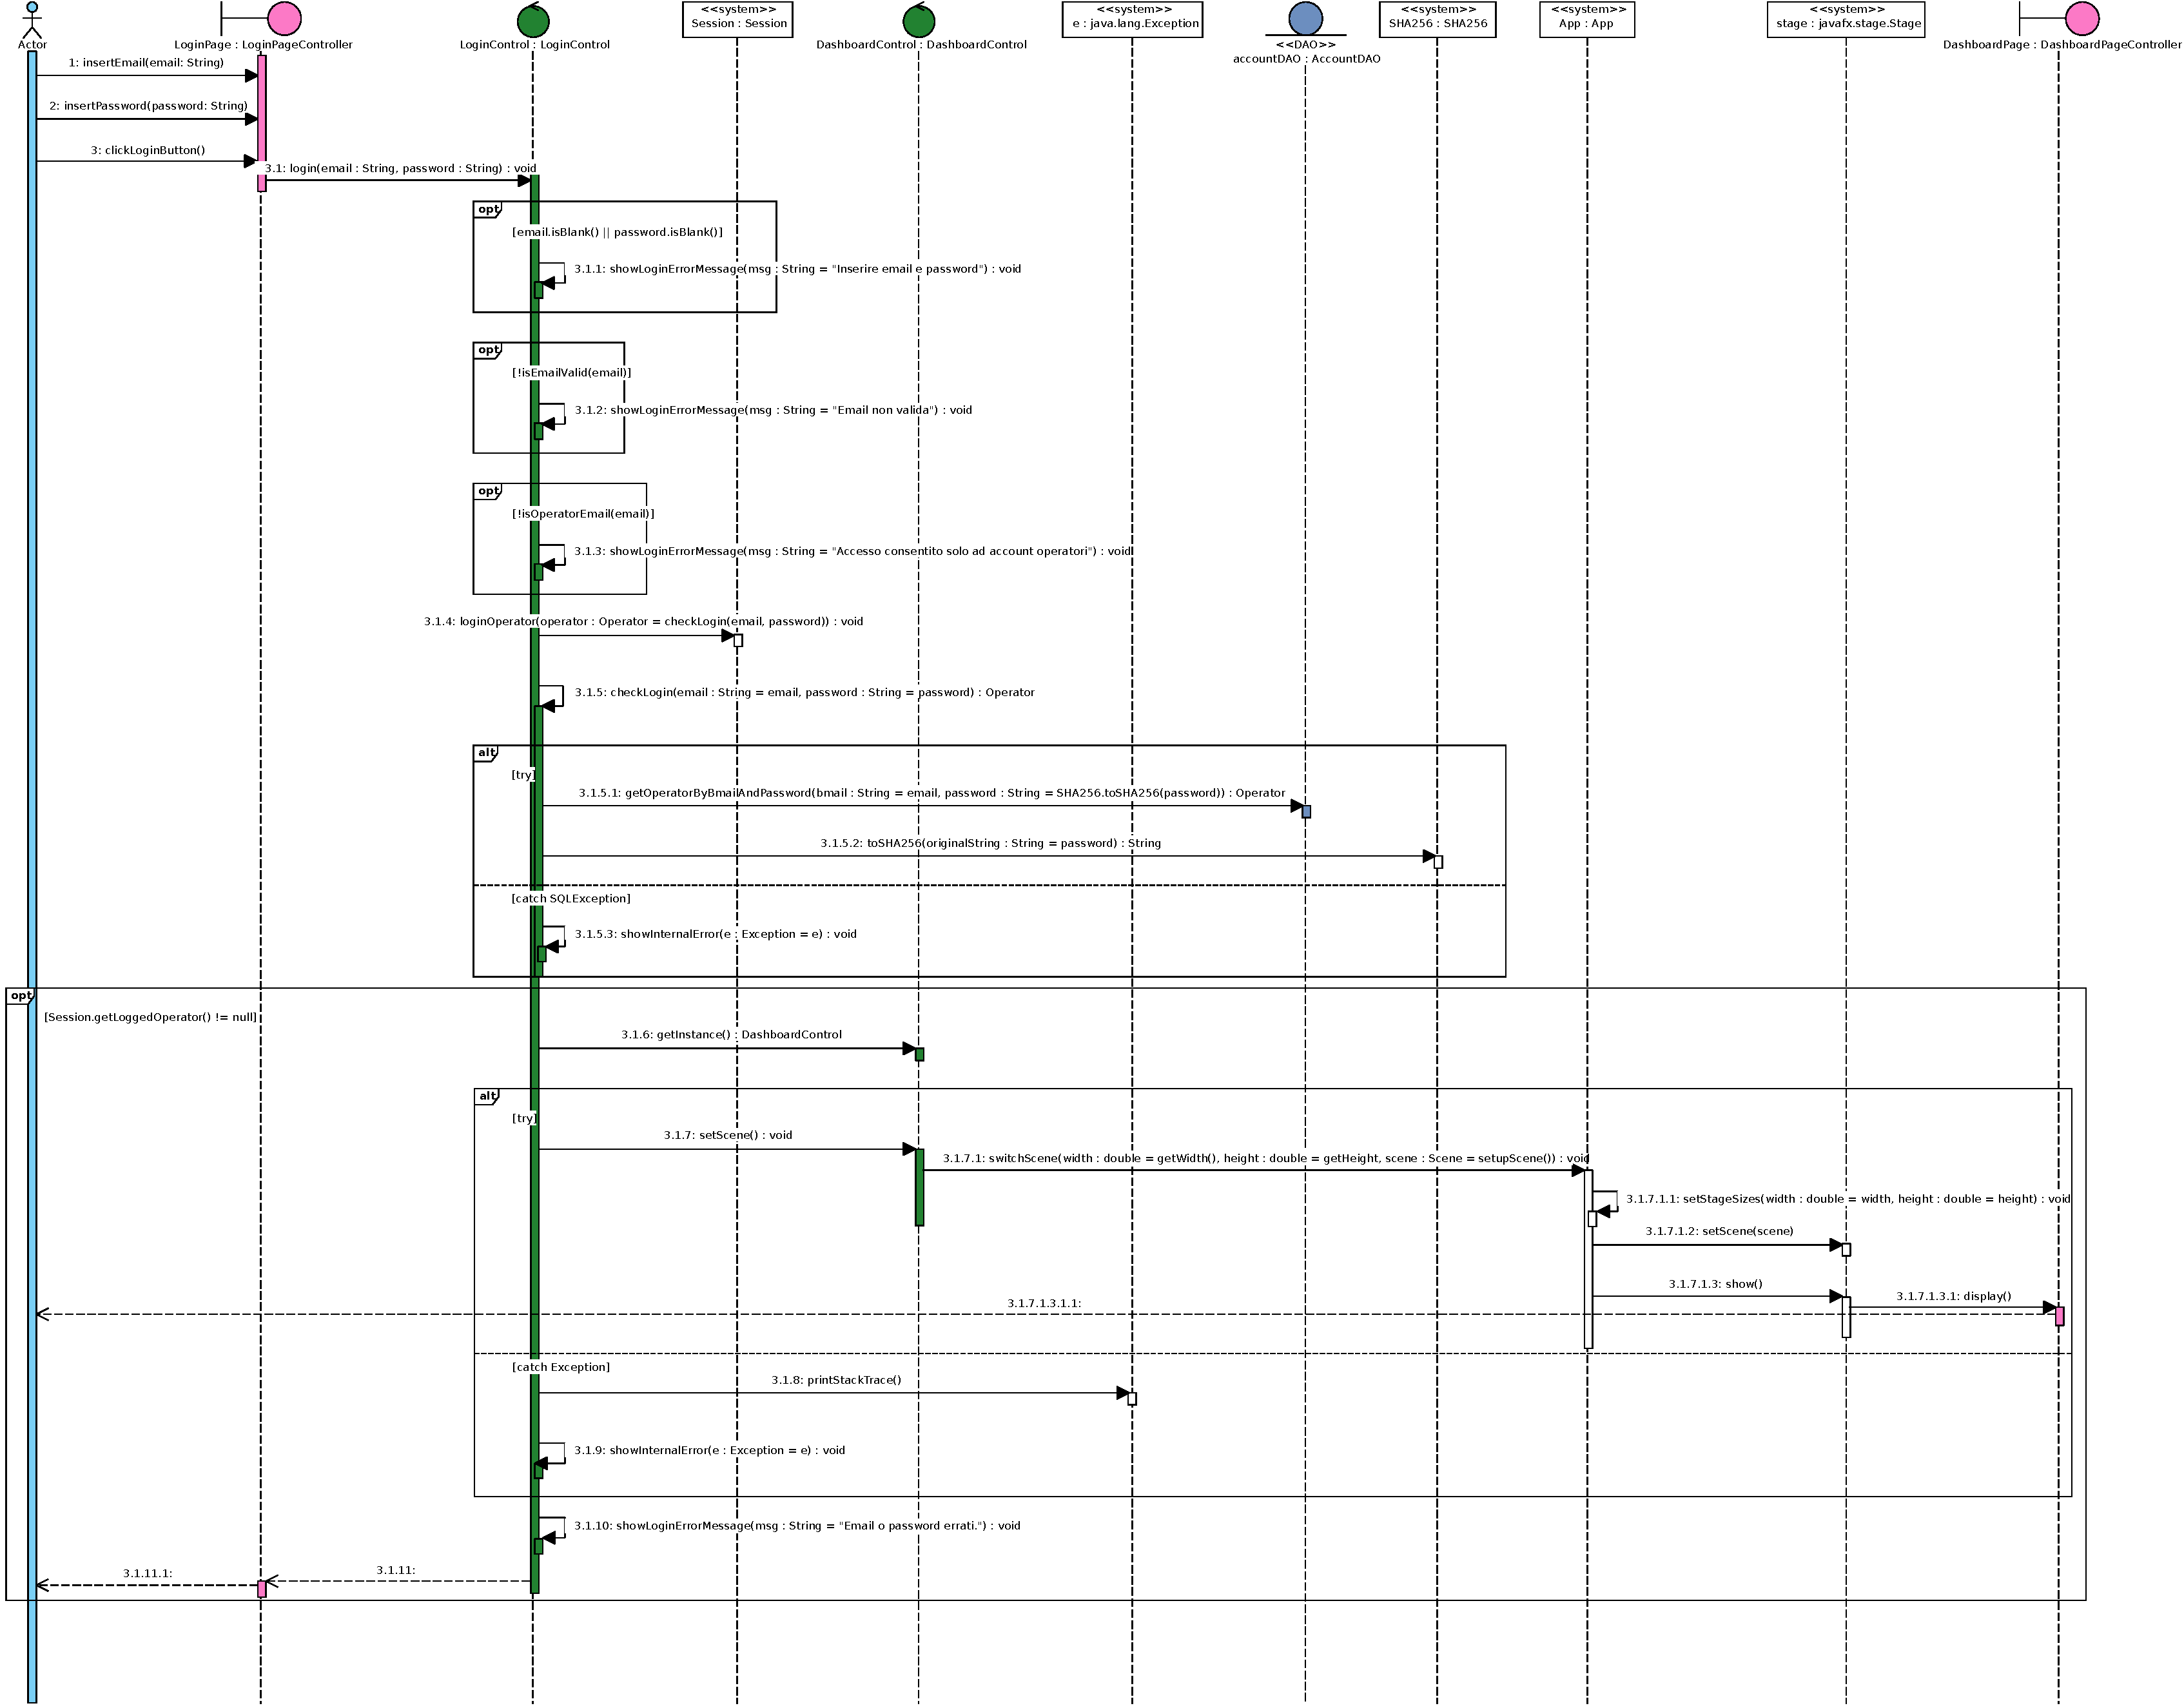
\includegraphics[width=\textwidth]{sequenceDiagrams/Login}
  \caption{Sequence Diagram --- Login}
\end{figure}

\newpage

\section{Spedizione degli ordini}

\begin{figure}[H]
  \centering
  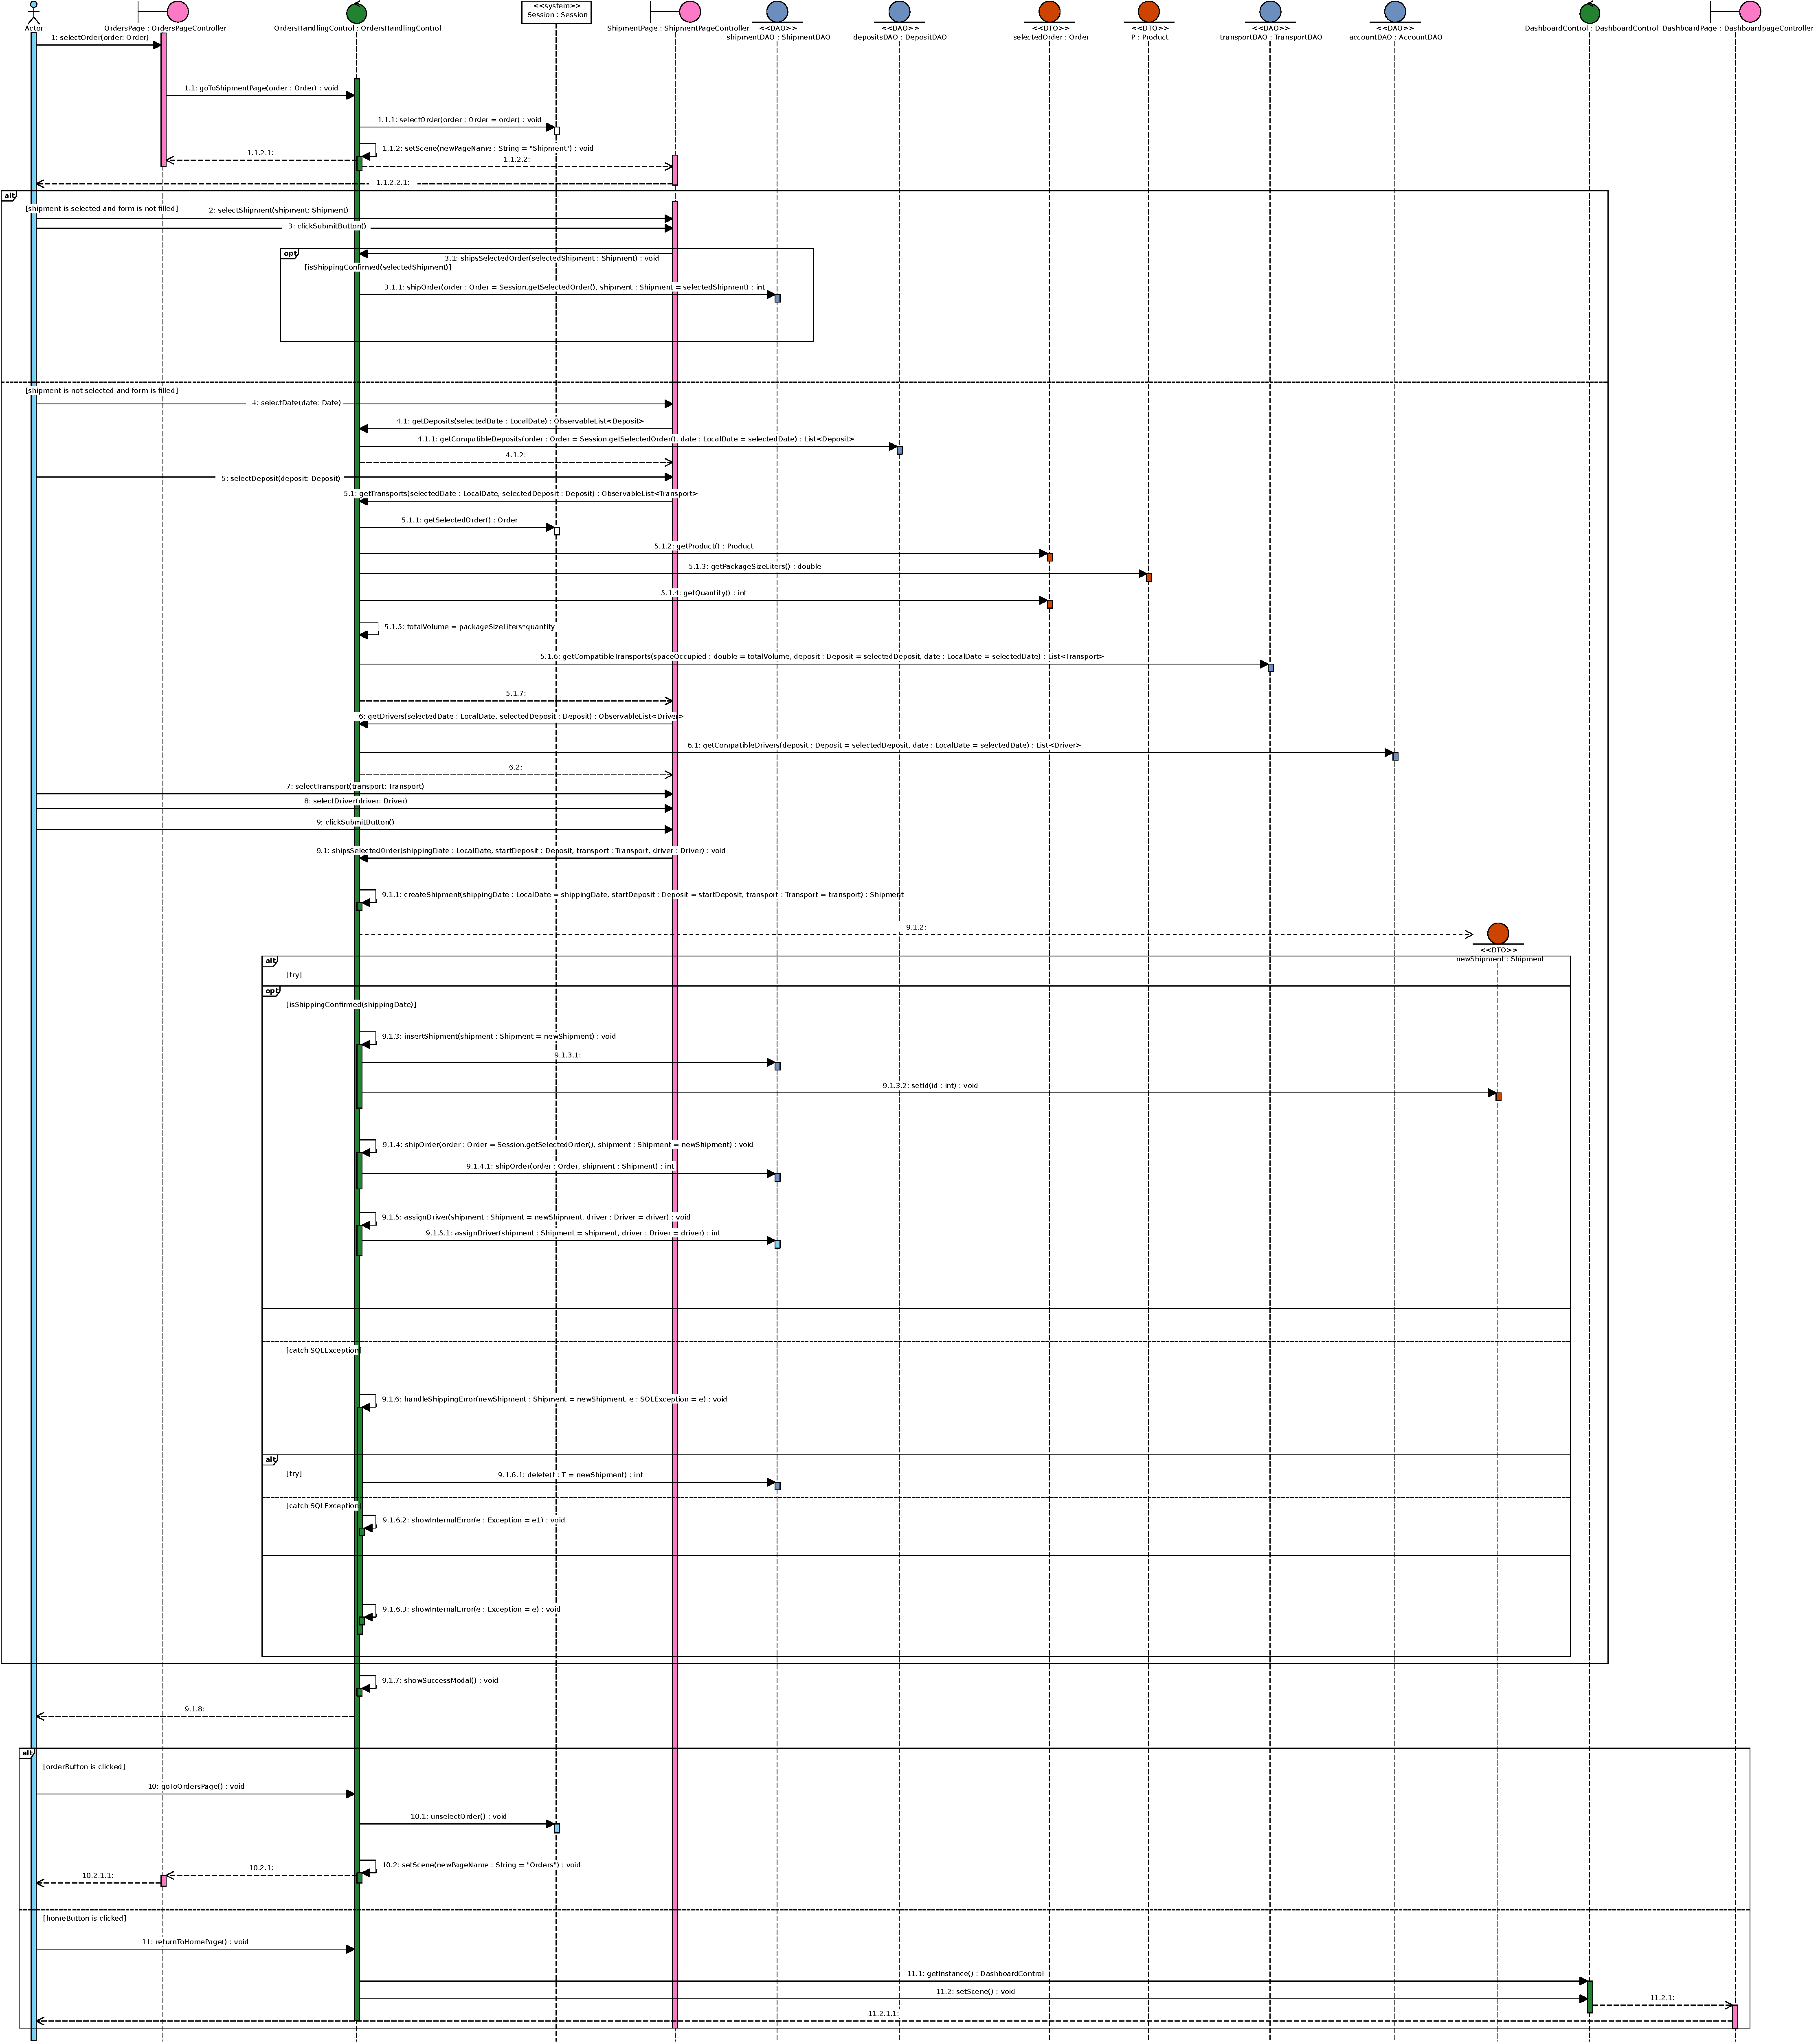
\includegraphics[width=\textwidth]{sequenceDiagrams/orderShipment}
  \caption{Sequence Diagram --- Spedizione degli ordini}
\end{figure}

